\documentclass[twoside,11pt]{article}

% Any additional packages needed should be included after jmlr2e.
% Note that jmlr2e.sty includes epsfig, amssymb, natbib and graphicx,
% and defines many common macros, such as 'proof' and 'example'.
%
% It also sets the bibliographystyle to plainnat; for more information on
% natbib citation styles, see the natbib documentation, a copy of which
% is archived at http://www.jmlr.org/format/natbib.pdf

\usepackage{jmlr2e}

% Definitions of handy macros can go here

\newcommand{\dataset}{{\cal D}}
\newcommand{\fracpartial}[2]{\frac{\partial #1}{\partial  #2}}

% Short headings should be running head and authors last names

\ShortHeadings{CS273B Final Research Project Report}{Ganesh, Pourshafeie, Ghorbani, Hwang, Yang and Liu}
\firstpageno{1}

\begin{document}

\title{Deep recurrent sequence-to-sequence learning for chromatin profile prediction}

\author{\name Adithya Ganesh \\
		\name Armin Pourshafeie \\
        \name Behrooz Ghorbani \\
        \name Philip Hwang \\
        \name Karen Yang \\
        \name Wendi Liu}

\editor{}

\maketitle

\begin{abstract}%   <- trailing '%' for backward compatibility of .sty file
We consider de novo prediction of Chromatin profile using deep neural networks. To take long-range correlations into consideration, we choose a LSTM-architecture for this task. We show how already discovered motifs can be leveraged to improve the prediction. We compare the performance of our model with DeapSea [cite ] and 
% * <ghorbani@stanford.edu> 2016-11-17T19:01:23.366Z:
%
% This is very nice but usually it comes in the introduction rather than abstract
%
% ^.
% Understanding the functionality of non-coding genomic variants is of paramount importance, as the majority of disease-associated variants lie in these regions [Citation Needed / we can mention 93 percent].  Various research works have developed scoring methods, such as CADD [3] and PolyPhen [4], that aim to quantify the pathogenicity of a variant. These algorithms largely rely on population-dependent statistics, such as alternate allele frequencies.
\end{abstract}

\begin{keywords}
  %Sequence-to-sequence Learning, 
  Chromatin Profile Prediction
\end{keywords}

\section{Introduction}
Recently, Zhou et al. \cite{zhou2015predicting} and Quang et al. \cite{quang2016danq} applied a deep learning method to predict chromatin profile {\it de novo}, using only sequence information. The predicted chromatin profile can then be used to model functional effects.  The DeepSEA model [1]  uses three convolutional layers which serve as spatial motif detectors.  The DanQ model [2] replaces this architecture with a single convolutional layer followed by a bi-directional LSTM.  This recurrent structure can model long-term dependencies between distant portions of the input sequence.  Both methods are able to compute a predicted chromatin profile from a 200-bp window surrounded by 800-bp of additional context.

However, both of these methods employ convolutional layers, they both require a fixed input length (in this case 1000-bp).  Zhou et al. [1] have demonstrated that training DeepSEA models with inputs of larger context size results in increased prediction accuracy (see Figure \ref{fig:context-acc}). This observation is consistent with the fact that distant motifs are known to exhibit co-dependent behavior.  In certain cases, regulatory sites can be kilobases or even megabases away from the target gene.  Using a deep learning architecture that is fully recurrent will allow us to model these very distant dependencies.

\subsection{Architecture}
An extension of the Long Short-Term Memory (LSTM) architecture, {\it sequence to sequence learning} [5], can be applied to model general sequence to sequence problems.  This method consists of two deep recurrent neural networks,  namely:

\begin{itemize}
\item an encoder network that processes the input and obtains a fixed-length representation
\item a decoder network that generates the output of arbitrary length
\end{itemize}

This approach and related ones have been applied in [5], [6], and [7] and has achieved state-of-the-art results in machine translation and speech recognition tasks.  A graphical representation of this architecture can be seen in Figure \ref{fig:seq2seq}.

\begin{figure}[!htbp]
\centering
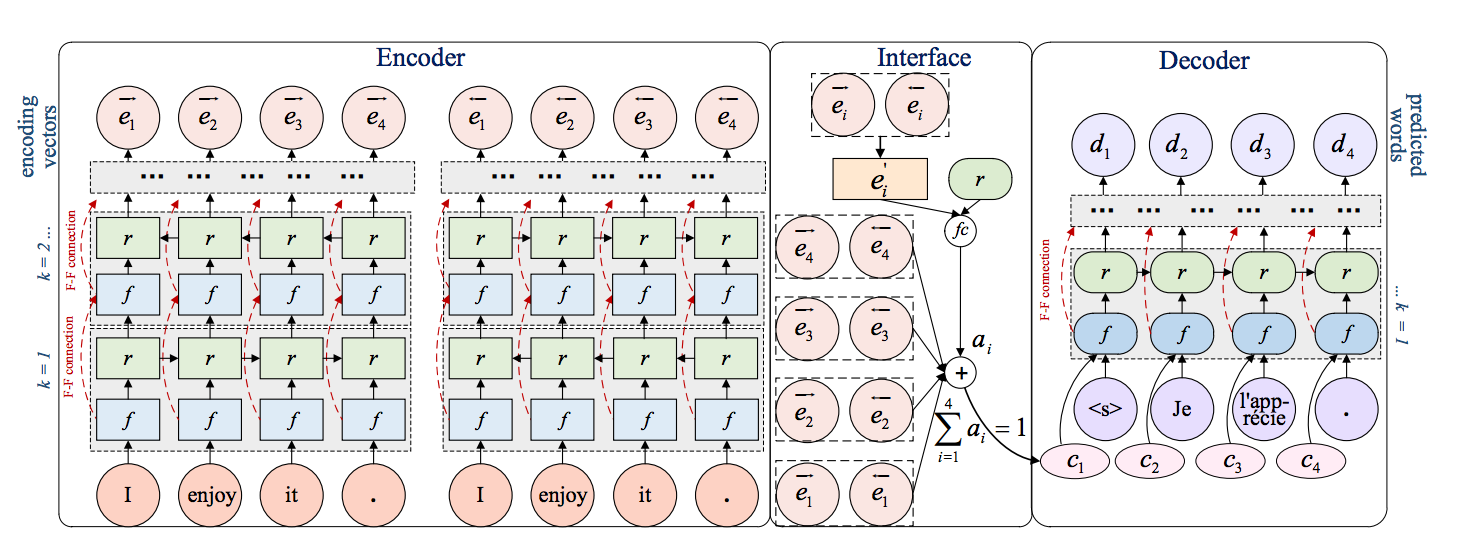
\includegraphics[width=\textwidth]{seq2seq_b.png}
\caption{Graphical representation of sequence to sequence learning, using the example Deep-Att [8] architecture in a machine translation setting}
\label{fig:seq2seq}
\end{figure}

Our objective is to compare the performance of two strategies.  First, we will use the sequence to sequence framework in the multi-task setting, to learn chromatin profiles directly from sequence (see Figure \ref{fig:approach1}).

\begin{figure}[!htbp]
\centering
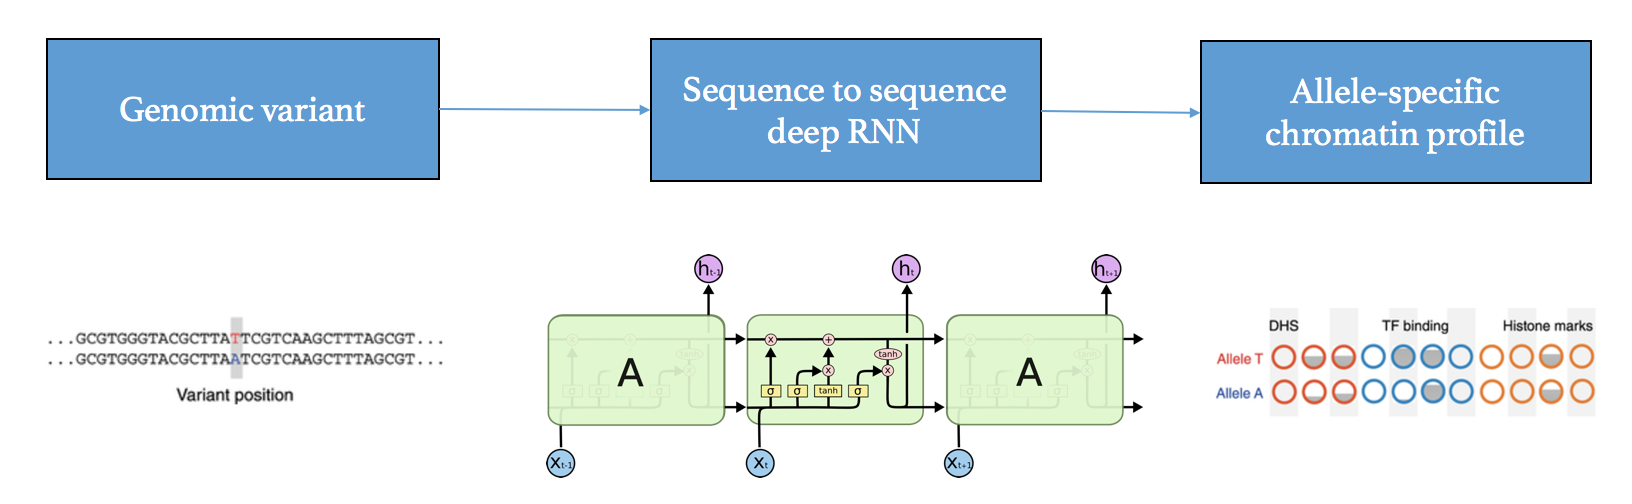
\includegraphics[width=\textwidth]{model1.png}
\caption{Approach A: Directly predicting allele-specific chromatin profile from variant}
\label{fig:approach1}
\end{figure}

Both DeepSEA and DanQ take advantage of CNNs as a motif discovery tool, due to their powerful modeling capacity for spatial features.  We anticipate that a fully recurrent architecture may not be as effective as discovering motifs.  As a second strategy, we will first convert a genomic variant to a matrix of ``motif scores.''  Subsequently, we will train a sequence-to-sequence RNN model on this motif-encoded sequence (see Figure \ref{fig:approach2}.)

\begin{figure}[!htbp]
\centering
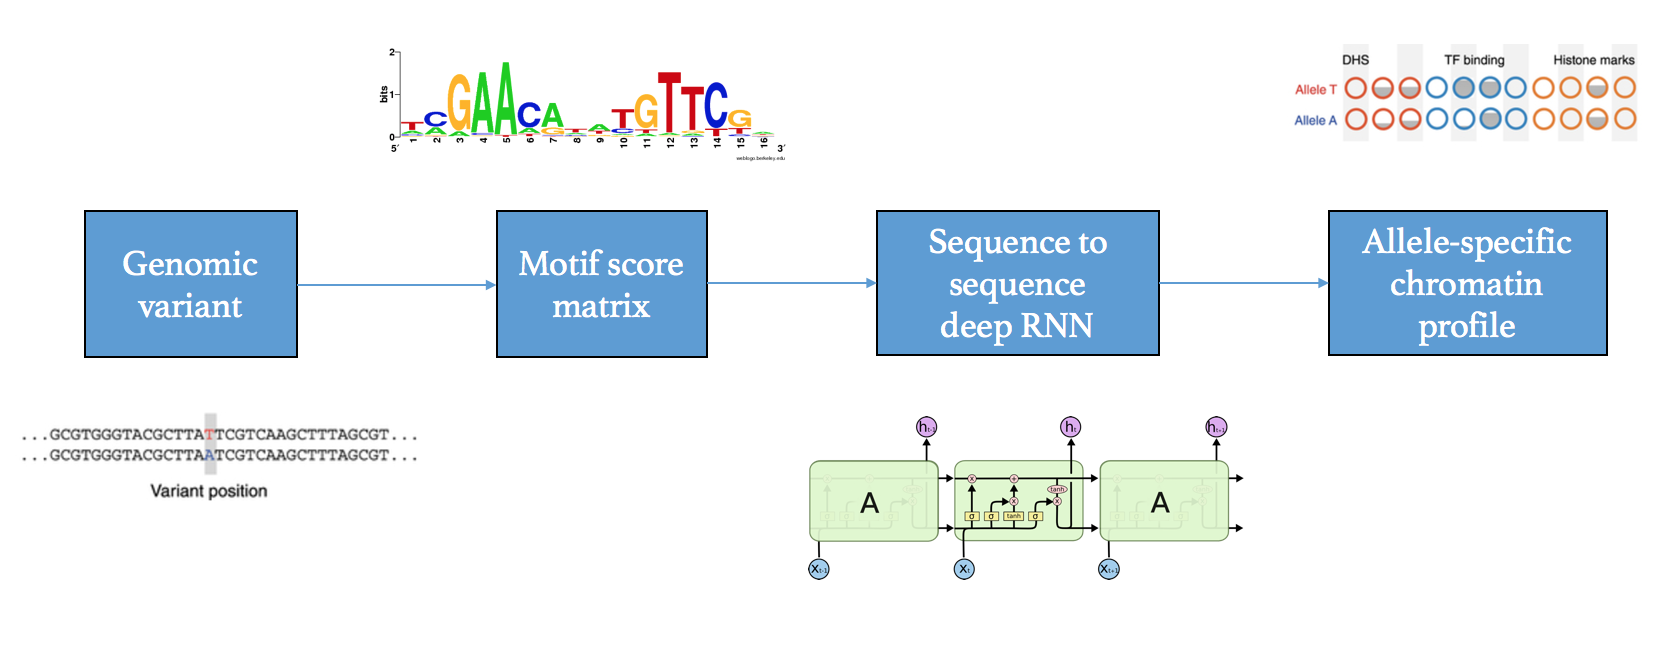
\includegraphics[width=\textwidth]{model2.png}
\caption{Approach B: Computing a motif score matrix and then applying sequence to sequence learning}
\label{fig:approach2}
\end{figure}

In order to benchmark our approach against published algorithms, we will use chromatin profile data used by Zhou et al. [1].  We will use PR-AUC and ROC-AUC as performance metrics for chromatin profile prediction and we will benchmark our method against both the DeepSEA and DanQ models.

% Acknowledgements should go at the end, before appendices and references

\acks{We would like to acknowledge support for this project
from the National Science Foundation (NSF grant IIS-9988642)
and the Multidisciplinary Research Program of the Department
of Defense (MURI N00014-00-1-0637). }

% Manual newpage inserted to improve layout of sample file - not
% needed in general before appendices/bibliography.

\newpage

\appendix
\section*{Appendix A.}
\label{app:theorem}

% Note: in this sample, the section number is hard-coded in. Following
% proper LaTeX conventions, it should properly be coded as a reference:

%In this appendix we prove the following theorem from
%Section~\ref{sec:textree-generalization}:

In this appendix we prove the following theorem from
Section~6.2:

\noindent
{\bf Theorem} {\it Let $u,v,w$ be discrete variables such that $v, w$ do
not co-occur with $u$ (i.e., $u\neq0\;\Rightarrow \;v=w=0$ in a given
dataset $\dataset$). Let $N_{v0},N_{w0}$ be the number of data points for
which $v=0, w=0$ respectively, and let $I_{uv},I_{uw}$ be the
respective empirical mutual information values based on the sample
$\dataset$. Then
\[
	N_{v0} \;>\; N_{w0}\;\;\Rightarrow\;\;I_{uv} \;\leq\;I_{uw}
\]
with equality only if $u$ is identically 0.} \hfill\BlackBox

\noindent
{\bf Proof}. We use the notation:
\[
P_v(i) \;=\;\frac{N_v^i}{N},\;\;\;i \neq 0;\;\;\;
P_{v0}\;\equiv\;P_v(0)\; = \;1 - \sum_{i\neq 0}P_v(i).
\]
These values represent the (empirical) probabilities of $v$
taking value $i\neq 0$ and 0 respectively.  Entropies will be denoted
by $H$. We aim to show that $\fracpartial{I_{uv}}{P_{v0}} < 0$....\\

{\noindent \em Remainder omitted in this sample. See http://www.jmlr.org/papers/ for full paper.}


\vskip 0.2in
\bibliography{Bibliography}

\end{document}